
\subsection{Analytical solution}

\subsubsection{Analytical solution for \texorpdfstring{$\mathrm{Pe} = \infty$}{infinite Péclet's number}}

As we have previously seen, Péclet's number is defined as
\begin{equation}
	\mathrm{Pe} = 
	\frac{\text{convection transport rate}}{\text{diffusion transport rate}} = 
	\frac{\rho u L}{\Gamma}
\end{equation}
Whenever $\mathrm{Pe} \to +\infty$, it implies $\Gamma \to 0^+$ since infinite values for the density, velocity or characteristic length make no physical sense. Therefore the difussion coefficient tends to $0$, which means the Laplacian term, linked to the diffusion process, is negligible. Under this physical intuition, dividing the PDE from \eqref{eq:diagonal_case_cauchy_problem} results in the following Cauchy problem:
\begin{equation} \label{eq:diagonal_case_cauchy_problem_infinite_peclet}
	\left\{
	\begin{aligned}
		&\pdv{\phi}{x} + \pdv{\phi}{y} = 0 &
		&\text{in } \Omega = (0,L) \times (0,L) \\
		&\phi = \phi_\text{low} &
		&\text{on } C_1 = [0,L) \times \{ 0 \} \cup \{ L \} \times [0,L) \\
		&\phi = \phi_\text{high} &
		&\text{on } C_2 = \{ 0 \} \times (0,L] \cup (0,L] \times \{ L \}
	\end{aligned}
	\right.
\end{equation}
The PDE from \eqref{eq:diagonal_case_cauchy_problem_infinite_peclet} is known as the transport equation, which is a first order linear PDE. In our case it has constant coefficients, making it easier to solve analitically. So as to find the analytical solution to \eqref{eq:diagonal_case_cauchy_problem_infinite_peclet}, we will follow a geometric approach as it is more intuitive. 

A classical solution to \eqref{eq:diagonal_case_cauchy_problem_infinite_peclet} is a function $\phi \colon \overline{\Omega} \rightarrow \real$ such that:
\begin{enumerate}[label={(\roman*)}, topsep=0pt]
	\item $\phi \in \mathcal{C}^1(\Omega) \cap \mathcal{C}(\overline{\Omega})$, \ie $\phi$ is differentiable with continuity in $\Omega$ and continuous up to the boundary,
	\item $\phi$ satisfies the PDE, and
	\item $\phi$ satisfies the boundary conditions.
\end{enumerate}
In order to find the solution to \eqref{eq:diagonal_case_cauchy_problem_infinite_peclet}, we will assume $\phi$ is a $\mathcal{C}^1(\Omega) \cap \mathcal{C}(\overline{\Omega})$ function. Once we find the solution, we will be able to tell whether $\phi$ is a classical solution, or otherwise give a meaning to $\phi$.

We introduce some notation which will be useful. Given $m$ vectors $\vb{w}_1, \ldots, \vb{w}_m \in \real^n$, the set $[\vb{w}_1, \ldots, \vb{w}_m] = \{ \sum_{i=1}^m \lambda_i \vb{w}_i \mid \lambda_1, \ldots, \lambda_m \in \real \}$ is the vector subspace of $\real^n$ spanned by $\vb{w}_1, \ldots, \vb{w}_m$. If $W \subset \real^m$ is a vector subspace, $W^\perp = \{ v \in \real^n \mid v \vdot w = 0 \ \forall w \in W \}$ is the vector subspace orthogonal to $W$.

So as to deduce the solution to \eqref{eq:diagonal_case_cauchy_problem_infinite_peclet}, we shall follow the method of characteristics. Using the gradient of $\phi$ we can write the PDE as
\begin{equation} \label{eq:diagonal_case_cauchy_problem_infinite_peclet_orthogonal_vectors}
	\left( 1, 1 \right)
	\vdot
	\grad{\phi} = 
	\left( 1, 1 \right)
	\vdot
	\begin{pmatrix}
	\displaystyle\pdv{\phi}{x} \\[10pt] \displaystyle\pdv{\phi}{y}
	\end{pmatrix} = 
	\pdv{\phi}{x} + \pdv{\phi}{y} = 0
\end{equation}
Recall from vector calculus that the gradient vector of $\phi$, $\grad{\phi} = \left( \pdv{\phi}{x}, \pdv{\phi}{y} \right)^T \in \real^2$, gives the direction of maximum growth of $\phi$ at each point, whilst a non--zero vector $\vb{w} \in [\grad{\phi}]^\perp$ provides the direction through which $\phi$ remains constant. Equation \eqref{eq:diagonal_case_cauchy_problem_infinite_peclet_orthogonal_vectors} tells us than $\phi$ is constant along the direction given by $(1, 1)$. To check this, we may exploit the fact that the PDE is first--order linear and use the chain rule to rewrite \eqref{eq:diagonal_case_cauchy_problem_infinite_peclet_orthogonal_vectors}. Let $I \subset \real$ be an open interval and let $g \equiv (g_1, g_2) \colon I \subset \real \rightarrow \Omega \subset \real^2$, $s \mapsto g(s) = (g_1(s), g_2(s))$ be a $\mathcal{C}^1$ mapping such that $g_1' = g_2' = 1$. The image of $g$, $C = \image{g} = \{ (x, y) \in \real^2 \mid x = g_1(s), \, y = g_2(s), \, s \in I \} \subset \Omega$ is a $\mathcal{C}^1$ curve in $\real^2$. The restriction of $\phi$ to $g$, given by $\varphi = \phi \circ g \colon \real \rightarrow \real$, is also a $\mathcal{C}^1$ function. By the chain rule,
\begin{equation} \label{eq:diagonal_case_cauchy_problem_infinite_peclet_chain_rule}
	\frac{\dd}{\dd{s}} \varphi(s) = 
	\frac{\dd}{\dd{s}} \phi(g_1(s), g_2(s)) = 
	\frac{\partial \phi}{\partial x} (g_1(s), g_2(s)) \, g_1'(s) + 
	\frac{\partial \phi}{\partial y} (g_1(s), g_2(s)) \, g_2'(s) =
	\frac{\partial \phi}{\partial x} + \frac{\partial \phi}{\partial y} = 0
\end{equation}
which implies that $\varphi$ is a constant function on $I$, that is to say, $\phi$ is constant along the curve $C \subset \Omega$. Now we would like to find the curve $C$. By hypothesis, we have $g_1' = g_2' = 1$. Moreover, the component functions of $g$ can be interpreted as the coordinates of a point in $\real^2$, that is $(g_1(s), g_2(s)) = (x, y)$. Given this information, we can pose the following Cauchy problem:
\begin{equation} \label{eq:diagonal_case_cauchy_problem_infinite_peclet_characteristics_problem}
	\left\{
	\begin{aligned}
		&g'(s) = (g_1'(s), g_2'(s)) = (1, 1) & &\text{in } I \subset \real \\
		&g(0) = (g_1(0), g_2(0)) = (x_0, y_0)
	\end{aligned}
	\right.
\end{equation}
The solution to \eqref{eq:diagonal_case_cauchy_problem_infinite_peclet_characteristics_problem} exists and is unique due to \colorbox{red}{Teorema existencia y unicidad}, and is given by
\begin{equation}
	g(s) = (x_0 + s, y_0 + s) = (x_0, y_0) + s(1, 1)
\end{equation}
The point $(x_0, y_0) \in \real^2$ is arbitrary, but it should be chosen so that it eases finding the solution to \eqref{eq:diagonal_case_cauchy_problem_infinite_peclet}. Since part of the information of the solution is given by the boundary conditions, we may choose the point to be on the boundary. Therefore the curve along which $\phi$ is constant is not a single curve, but rather a family of curves given by
\begin{equation}
	G(s; x_0, y_0) = (x_0, y_0) + s(1, 1), \quad (x_0, y_0) \in \partial \Omega
\end{equation}
or in implicit form by the equation
\begin{equation} \label{eq:diagonal_case_cauchy_problem_infinite_peclet_characteristics_implicit_form}
	x - y = x_0 - y_0, \quad (x_0, y_0) \in \partial \Omega
\end{equation}
These curves are named characteristic curves or simply characteristics. Some of them are represented in figure \ref{fig:diagonal_case_cauchy_problem_infinite_peclet_characteristics_problem}.

\begin{figure}[h]
	\centering
	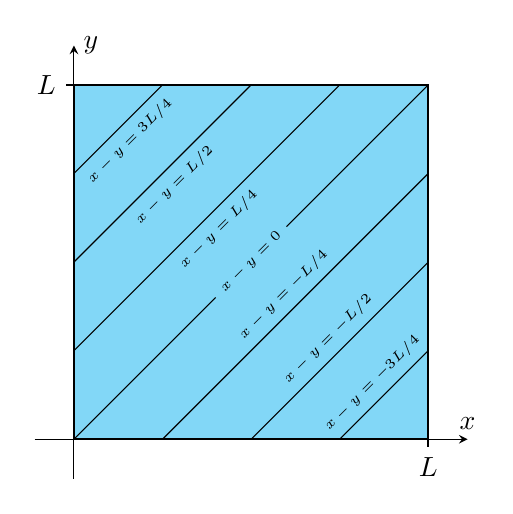
\begin{tikzpicture}
		% Lenghts
		\def\alength{5}
		\def\L{4.5}
		\def\mlength{0.1}
		% Axis
		\draw[-stealth] (0,-0.5) -- (0,\alength) node[right]{$y$};
		\draw[-stealth] (-0.5,0) -- (\alength,0) node[above]{$x$};
		\draw[black, thick] (\L,0) -- ++(0,-\mlength) node[below]{$L$};
		\draw[black, thick] (0,\L) -- ++(-\mlength,0) node[left]{$L$};
		% Domain
		\fill[cyan!70!white,opacity=0.7] (0,0) rectangle (\L, \L);
		\draw[thick, thick] (0,0) rectangle (\L, \L);
		% Characteristics
%		\draw[black] (0,0) -- node[midway, above, rotate=45]{\tiny{$x - y = 0$}} (\L, \L);
		\node[rotate=45] at ({0.5*\L}, {0.5*\L}) {\tiny{$x - y = 0$}};
		\draw[black] (0,0) -- ({0.4*\L}, {0.4*\L});
		\draw[black] ({0.6*\L}, {0.6*\L}) -- (\L, \L);
		
		\draw[black] ({0.25*\L}, 0) -- node[midway, above, rotate=45]{\tiny{$x - y = -L/4$}} 
		(\L, {0.75*\L});
		\draw[black] ({0.50*\L}, 0) -- node[midway, above, rotate=45]{\tiny{$x - y = -L/2$}} 
		(\L, {0.50*\L});
		\draw[black] ({0.75*\L}, 0) -- node[midway, above, rotate=45]{\tiny{$x - y = -3L/4$}} 
		(\L, {0.25*\L});
		
		
		
		\draw[black] (0, {0.25*\L}) -- node[midway, below, rotate=45]{\tiny{$x - y = L/4$}} 
		({0.75*\L}, \L);
		\draw[black] (0, {0.50*\L}) -- node[midway, below, rotate=45]{\tiny{$x - y = L/2$}} 
		({0.50*\L}, \L);
		\draw[black] (0, {0.75*\L}) -- node[midway, below, rotate=45]{\tiny{$x - y = 3L/4$}} 
		({0.25*\L}, \L);
	\end{tikzpicture}
	\caption{Some characteristics of problem \eqref{eq:diagonal_case_cauchy_problem_infinite_peclet}.}
	\label{fig:diagonal_case_cauchy_problem_infinite_peclet_characteristics_problem}
\end{figure}

\noindent
Intuitively, the characteristics give the paths in $\real^2$ through which the information of the boundary conditions is transported. Notice that each characteristic starting on $C_1$ ends on $C_1$, and the same is true for $C_2$. Moreover, by definition of the Cauchy problem, $\phi$ is constant on $C_1$ and on $C_2$. Using this and the fact that $\phi$ is constant on each characteristic, the solution to \eqref{eq:diagonal_case_cauchy_problem_infinite_peclet} is:
\begin{equation} \label{eq:diagonal_case_cauchy_problem_infinite_peclet_solution}
	\phi(x,y) = 
	\left\{
	\begin{aligned}
		&\phi_\text{low} & &\text{if } x - y \leq 0 \\
		&\phi_\text{high} & &\text{if } x - y > 0\\
	\end{aligned}
	\right.
	\quad
	(x, y) \in \overline{\Omega}
\end{equation}

Now we check our initial assumption that $\phi \in \mathcal{C}^1(\Omega) \cap \mathcal{C}(\overline{\Omega})$. If $\phi_\text{low} = \phi_\text{high}$ the solution \eqref{eq:diagonal_case_cauchy_problem_infinite_peclet_solution} is constant and therefore is a solution in the classical sense. Otherwise, we notice that $\phi$ is not continuous on the segment $\{ x - y = 0 \} \cap \overline{\Omega}$ whence it cannot be a differentiable function. 

\subsubsection{Analytical solution for \texorpdfstring{$\mathrm{Pe} = 0$}{zero Péclet's number}}

\subsubsection{General problem}